\documentclass[spec, och, otchet, hidelinks]{SCWorks}
% параметр - тип обучения - одно из значений:
%    spec     - специальность
%    bachelor - бакалавриат (по умолчанию)
%    master   - магистратура
% параметр - форма обучения - одно из значений:
%    och   - очное (по умолчанию)
%    zaoch - заочное
% параметр - тип работы - одно из значений:
%    otchet
%    referat    - реферат
%    coursework - курсовая работа (по умолчанию)
%    diploma    - дипломная работа
%    pract      - отчет по практике
%    pract      - отчет о научно-исследовательской работе
%    autoref    - автореферат выпускной работы
%    assignment - задание на выпускную квалификационную работу
%    review     - отзыв руководителя
%    critique   - рецензия на выпускную работу
% параметр - включение шрифта
%    times    - включение шрифта Times New Roman (если установлен)
%               по умолчанию выключен
\usepackage[T2A]{fontenc}
\usepackage[utf8]{inputenc}
\usepackage{graphicx}

\usepackage[sort,compress]{cite}
\usepackage{amsmath}
\usepackage{amssymb}
\usepackage{amsthm}
\usepackage{fancyvrb}
\usepackage{longtable}
\usepackage{array}
\usepackage{listings}
\usepackage[english,russian]{babel}
\usepackage{minted}
% Используется автором репозитория
%\usemintedstyle{xcode}
% Этот пакет включает в себя аналогичный Times New Roman шрифт.
% Необходим для успешной компиляции для UNIX-систем ввиду отсутствия TNR в нем.
% Можно использовать и для Windows.
\usepackage{tempora}

\lstdefinestyle{listingStyle}{%
	backgroundcolor=\color{gray!12},
	basicstyle=\ttfamily\small,
	keywordstyle=\color{magenta},
	stringstyle=\color{blue},
	showstringspaces=false,
	captionpos=b,
	numbers=left,
	numberstyle=\footnotesize\color{gray},
	frame=TB,
	tabsize=2
}


\usepackage[colorlinks=false]{hyperref}

\graphicspath{{figures/}}

\newcommand{\eqdef}{\stackrel {\rm def}{=}}

\usepackage{stackengine}
\newcommand\xrowht[2][0]{\addstackgap[.5\dimexpr#2\relax]{\vphantom{#1}}}

\newtheorem{lem}{Лемма}

% % При использовании biblatex вместо bibtex
%\usepackage[style=gost-numeric]{biblatex}
%\addbibresource{thesis.bib}

\begin{document}

% Кафедра (в родительном падеже)
\chair{математической кибернетики и компьютерных наук}

% Тема работы
\title{Сведение задачи об узельном покрытии к задаче о множестве рёбер, разрезающих циклы}

% Курс
\course{3}

% Группа
\group{331}

% Факультет (в родительном падеже) (по умолчанию "факультета КНиИТ")
%\department{факультета КНиИТ}

% Специальность/направление код - наименование
%\napravlenie{02.03.02 "--- Фундаментальная информатика и информационные технологии}
%\napravlenie{02.03.01 "--- Математическое обеспечение и администрирование информационных систем}
%\napravlenie{09.03.01 "--- Информатика и вычислительная техника}
%\napravlenie{09.03.04 "--- Программная инженерия}
\napravlenie{10.05.01 "--- Компьютерная безопасность}

% Для студентки. Для работы студента следующая команда не нужна.
%\studenttitle{Студентки}

% Фамилия, имя, отчество в родительном падеже
\author{Бородина Артёма Горовича}

% Заведующий кафедрой
\chtitle{доцент, к.\,ф.-м.\,н.} % степень, звание
\chname{С.\,В.\,Миронов}

%Научный руководитель (для реферата преподаватель проверяющий работу)
\satitle{к.\,ф.-м.\,н.} %должность, степень, звание
\saname{А.\,Н.\,Гамова}

% Руководитель практики от организации (только для практики,
% для остальных типов работ не используется)
\patitle{к.\,ф.-м.\,н., доцент}
\paname{Д.\,Ю.\,Петров}

% Семестр (только для практики, для остальных
% типов работ не используется)
\term{2}

% Наименование практики (только для практики, для остальных
% типов работ не используется)
\practtype{учебная}

% Продолжительность практики (количество недель) (только для практики,
% для остальных типов работ не используется)
\duration{2}

% Даты начала и окончания практики (только для практики, для остальных
% типов работ не используется)
\practStart{01.07.2016}
\practFinish{14.07.2016}

% Год выполнения отчета
\date{2022}

\maketitle

% Включение нумерации рисунков, формул и таблиц по разделам
% (по умолчанию - нумерация сквозная)
% (допускается оба вида нумерации)
%\secNumbering


\tableofcontents

% Раздел "Обозначения и сокращения". Может отсутствовать в работе
% \abbreviations
% \begin{description}
%     \item ... "--- ...
%     \item ... "--- ...
% \end{description}

% Раздел "Определения". Может отсутствовать в работе
%\definitions

% Раздел "Определения, обозначения и сокращения". Может отсутствовать в работе.
% Если присутствует, то заменяет собой разделы "Обозначения и сокращения" и "Определения"
%\defabbr


% Раздел "Введение"

\intro

Целью данной лабораторной работы служит рассмотрение вопроса сводимости задачи о вершинном покрытии к задаче о нахождении множества рёбер, разрезающих 
циклы. Для сведённой задачи требуется осуществить программную реализацию с эффективной (полиномиальной) временной сложностью.

\newpage

\section*{Решение вопроса сводимости}
\addcontentsline{toc}{section}{Решение вопроса сводимости}

\textbf{Теорема.} Задача об узельном покрытии полиномиально
трансформируема (сводима) в задачу о множестве рёбер, разрезающих циклы. Поэтому задача о множестве рёбер, разрезающих циклы, NР-полна.
\par \textbf{Доказательство.} Пусть $G=(V, E)$ -- неориентирован­ный граф, а $D = (V \times \{ 0, 1\}, \, E^{\prime}) $ -- ориентированный граф, где $E'$ состоит из 

\par 1) $[v, 0] \rightarrow [v, 1]$ для каждого $v \in V$ и

\par 2) $[v, 1] \rightarrow [w, 0]$ и $[w, 1] \rightarrow [v, 0]$ для каждого неориентирован­ного ребра $(v, w) \in E$.

\par Пусть $F \subset E'$ -- множество ребер графа $D$, содержащих по край­ней мере одно ребро из каждого цикла в $D$. Заменим каждое ребро из $F$, 
имеющее вид $[v, 1] \rightarrow [w, 0]$, ребром $[w, 0] \rightarrow [w, 1]$. Полученное множество обозначим через $F'$ . Утверждается, что $|F'| \leq 
|F|$ и $F'$ содержит по крайней мере одно ребро из каждого цикла (единственное ребро, выходящее из $[w, 0],$ идёт в $[w, 1],$ так что $[w, 0] \rightarrow
[w, 1]$ принадлежит любому циклу, содержащему $[v, 1] \rightarrow [w, 0]).$

\begin{figure}[h]
	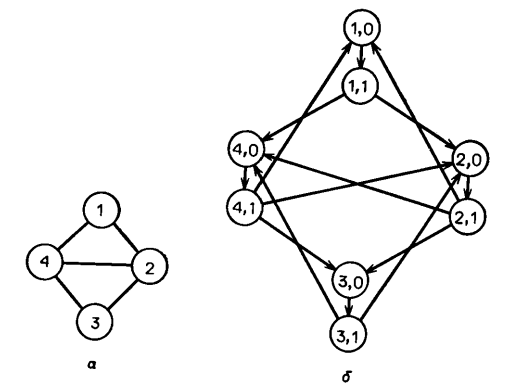
\includegraphics[scale=0.9]{graphs.png}
	\caption{\textbf{а} -- неориентированный граф \textit{G}; \textbf{\text{б}} -- соответствующий ориентированный граф \textit{D}. Узельное покрытие 
	{2, 4} соответствует множеству {[2, 0] $\rightarrow$ [2, 1], [4, 0] $\rightarrow$ [4, 1]} рёбер, разрезающих циклы.}
\end{figure}

\newpage

Ради общности, будем считать, что
$$F' = \{[v_i, 0] \rightarrow [v_i, 1] \; | \; 1 \leq i \leq k \} $$
для некоторого $k$. Тогда каждый цикл в $D$ содержит ребро $[v_i, 0] \rightarrow [v_i, 1]$ для некоторого $i, \; 1 \leq i \leq k$. Заметим, что если 
$(x, y)$ -- произвольное ребро в $G$, то $[x, 1], [y, 0], [y, 1], [x, 0], [x, 1]$ образуют цикл в $D$. Поэтому каждое ребро в $G$ инцидентно некоторому
узлу $v_i, \; 1 \leq i \leq k,$ и, значит, ${v_1, \dots, v_k}$ -- узельное покрытие графа $G$.

\par Обратно, можно показать, что если $S$ -- узельное покрытие размера $k$, то $\{[v, 0] \rightarrow [v, 1] \; | \; v \in S\}$ -- множество ребер, 
разрезаю­щих циклы в $D$. Чтобы узнать, содержит ли $G$ узельное покрытие размера $k$, надо построить за полиномиальное время граф $D$ и выяснить, 
есть ли в нем $k$-элементное множество ребер, разрезающих циклы. $\square$

\newpage

\section*{Программная реализация}
\addcontentsline{toc}{section}{Программная реализация приближённого алгоритма}

\par Сначала приведём обоснование алгоритма. Пусть есть ориентированный граф $G$ и множество его вершин упорядочено: $v_1, v_2, \dots, v_n$. Будем 
называть такую перестановку \textit{последовательностью вершин} и обозначать $s = v_1v_2\dots v_n$. Каждая последовательность вершин $s$ порождает 
набор рёбер, разрезающих циклы $R(s)$, состоящий из всех дуг вида $v_jv_i, \, j > i$. Более того, каждому разрезающему циклы набору рёбер соответствует
некоторая последовательность вершин. Таким образом, задача поиска множества рёбер, разрезающих циклы эквивалентна поиску такой последовательности вершин $s$, что $R(s) = R(G)$.

\par \textbf{Алгоритм GR}. Алгоритм жадным образом удаляет из $G$ вершины (и инцидентные им рёбра), которые являются стоками или истоками или 
удовлетворяют следующему свойству: пусть для всякой вершины $u \in V \; d(u)$ обозначает степень $u, \; d^{+}(u) $ -- степень исхода, а $d^{-}(u)$ -- 
степень входа. Тогда $d(u) = d^{+}(u) + d^{-}(u)$. На каждом шаге работы алгоритма после удаления стоков и истоков удаляется единственная вершина, для 
которой $\delta(u) = d^{+}(u) - d^{-}(u)$ максимально. Если удалённая вершина $u$ является стоком, то она добавляется в последовательность вершин $s_2$;
иначе, $u$ добавляется в последовательность вершин $s_1$. Алгоритм работает до тех пор, пока из графа не будут удалены все его вершины. Результирующая
последовательность вершин получается как результат конкатенации последовательностей $s_1$ и $s_2$.

\begin{lstlisting}[caption=Алгоритм GR.,style=listingStyle, mathescape=true]
$\textbf{procedure}$ GR (G : DiGraph; var s : VertexSequence);
$s_1 \leftarrow \emptyset; \; s_2 \leftarrow \emptyset$
$\textbf{while} \;\, G \neq \emptyset \;\, \textbf{do}$
	{$\textbf{while} \;\, G \;\, \text{содержит сток} \;\, \textbf{do}$
			{$ \text{выбрать сток} \;\, u; \;\, s_2 \leftarrow us_2; \;\, G \leftarrow G - u$};
	 $\textbf{while} \;\, G \;\, \text{содержит исток} \;\, \textbf{do}$
	 		{$\text{выбрать исток} \;\, u; \;\, s_1 \leftarrow s_1u; \;\, G \leftarrow G - u$};
	 $\text{выбрать вершину} \;\, u, \;\, \text{для которой} \;\, \delta(u) \;\, \text{максимально}$;
	 $ \textbf{if} \;\, (u \;\, \text{-- сток}) \;\, s_2 \leftarrow us_2 $
	 $ \textbf{else} \;\, s_1 \leftarrow s_1u$;
	 $G \leftarrow G - u$;}
$s \leftarrow s_1s_2$.

\end{lstlisting}

\newpage

\par По заданному псевдокоду реализуем программу:

\begin{lstlisting}[caption=Программная реализация алгоритма GR.,style=listingStyle, mathescape=true, language=C++]
#include <iostream>
#include <vector>
#include <algorithm>
	
using namespace std;
	
int numberOfVertices, numberOfEdges;
vector<vector<int>> graph;
vector<int> vertices;
	
void displayGraphMatrix (vector<vector<int>> matrix)
{
	int i, j;
		
	for (i = 0; i < matrix.size (); ++i)
	{
		for (j = 0; j < matrix[i].size (); ++j)
		cout << matrix[i][j] << " ";
		cout << "\n";
	}
}
	
void getGraphMatrix ()
{
	int i, u, v;
		
	cout << "Input the number 
	         of vertices and the number of edges: ";
	cin >> numberOfVertices >> numberOfEdges;
	graph.assign (numberOfVertices, 
	              vector<int> (numberOfVertices, 0));
		
	cout << "Now input your edges:\n";
	for (i = 0; i < numberOfEdges; ++i)
	{
		cin >> u >> v;
		graph[--u][--v] = 1;
	}
}

bool inGraph (int vertex)
{
	int sumRow = 0, sumColumn = 0, i, 
	    negSize = graph.size () - 2 * graph.size ();
		
	for (i = 0; i < graph.size (); ++i)
		sumRow += graph[vertex][i], sumColumn += graph[i][vertex];
		
	return (!((sumRow == sumColumn) && (sumColumn == negSize)));
}
	
int extractSink (vector<vector<int>> matrix)
{
	int i, j;
	bool has_sink;
		
	for (i = 0; i < matrix.size (); ++i)
	{
		has_sink = true;
		for (j = 0; j < matrix[i].size (); ++j)
			if (matrix[i][j] == 1)
			{
				has_sink = false;
				break;
			}
		if (has_sink && inGraph (i))
			return (i);
	}
	return (-1);
}
	
void reduceMatrix (int vertex)
{
	int i;
		
	for (i = 0; i < graph.size (); ++i)
		graph[vertex][i] = graph[i][vertex] = -1;
}
	
int extractSource (vector<vector<int>> matrix)
{
	int i, j;
	bool has_source;
	
	for (i = 0; i < matrix.size (); ++i)
	{
		has_source = true;
		for (j = 0; j < matrix[i].size (); ++j)
		if (matrix[j][i] == 1)
		{
			has_source = false;
			break;
		}
		if (has_source && inGraph (i))
		return (i);
	}
	return (-1);
}
	
int getDelta (int vertex)
{
	int outdegree = 0, indegree = 0, i;
		
	for (i = 0; i < graph.size (); ++i)
	{
		if (graph[vertex][i] == 1)
		++outdegree;
		if (graph[i][vertex] == 1 && vertex != i)
		++indegree;
	}
	return (outdegree - indegree);
}
	
int getMaxDeltaVertex ()
{
	int maxDeltaVertex = 0, maxDelta = getDelta (0), i;
	
	for (i = 1; i < graph.size (); ++i)
	{
		int curDelta = getDelta (i);
		if (curDelta >= maxDelta && inGraph (i))
		maxDelta = curDelta, maxDeltaVertex = i;
	}
	return (maxDeltaVertex);
}
	
int adjacencySum ()
{
	int sum = 0, i, j;
	
	for (i = 0; i < graph.size (); ++i)
	for (j = 0; j < graph[i].size (); ++j)
	sum += graph[i][j];

	return (sum);
}
	
void feedbackArcSetProblem ()
{
	vector<int> seqOne, seqTwo;
	int vertexPlaceholder;
	getGraphMatrix ();
	int grSize = graph.size ();
	int negGrSizeSq = -(grSize * grSize);
		
	while (adjacencySum () != negGrSizeSq)
	{
		while ((vertexPlaceholder = extractSink (graph)) != -1)
		{
			seqTwo.push_back (vertexPlaceholder);
			reduceMatrix (vertexPlaceholder);
		}
		if (adjacencySum () == negGrSizeSq)
		break;
			
		while ((vertexPlaceholder = extractSource (graph)) != -1)
		{
			seqOne.push_back (vertexPlaceholder);
			reduceMatrix (vertexPlaceholder);
		}
		if (adjacencySum () == negGrSizeSq)
			break;
			
		vertexPlaceholder = getMaxDeltaVertex ();
		seqOne.push_back (vertexPlaceholder);
		reduceMatrix (vertexPlaceholder);
	}
	reverse (seqTwo.begin (), seqTwo.end ());
		
	cout << "\nThis is the first sequence (s_1): ";
	for (int vertex : seqOne)
		cout << ++vertex << " ";
	cout << "\n";
	cout << "This is the second sequence (s_2): ";
	for (int vertex : seqTwo)
		cout << ++vertex << " ";
	cout << "\n";
	cout << "This is the required sequence (s = s_1 + s_2): ";
	for (int vertex : seqOne)
		cout << ++vertex << " ";
	for (int vertex : seqTwo)
		cout << ++vertex << " ";
	cout << "\n";
	
	for (int i = 0; i < copyGraph.size (); ++i)
		for (int j = 0; j < copyGraph[i].size (); ++j)
		if (copyGraph[i][j] == 1)
			if (vertices[i] > vertices[j])
				cuttingEdges.push_back (make_pair (i, j));
	cout << "Cutting edges are: ";
	for (int i = 0; i < cuttingEdges.size (); ++i)
		cout << ++cuttingEdges[i].first << "-" << 
		        ++cuttingEdges[i].second << 
		        (i == cuttingEdges.size () - 1 ? "\n" : ", ");
	
}
	
int main ()
{
	feedbackArcSetProblem ();
		
	return (EXIT_SUCCESS);
}

\end{lstlisting}

\newpage 

\section*{Примеры запуска}

\par Рассмотрим результат работы программы на некоторых входных данных.

Пусть задан следующий граф:

\begin{figure}[h]
	\center{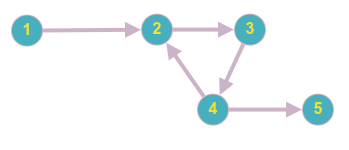
\includegraphics{prog_test/one_cycle_graph.png}}
	\caption{Некоторый граф, содержащий цикл.}
\end{figure}

Результатом работы программы должна быть последовательность вершин, позволяющая восстановить набор рёбер, разрезающих циклы. 

Результатом работы программы на этих входных данных будет являться следующая последовательность вершин и соответствующий ей набор рёбер, разрезающих циклы.

\begin{figure}[h]
	\center{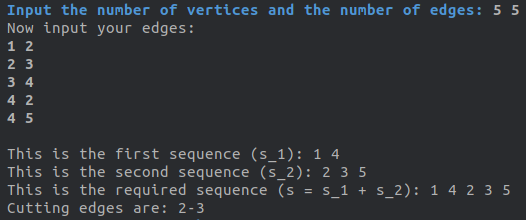
\includegraphics[scale=0.9]{prog_test/one_cycle_graph_output.png}}
	\caption{Полученная последовательность вершин и набор рёбер.}
\end{figure}

\newpage

Теперь рассмотрим граф с большим числом циклов:

\begin{figure}[h]
	\center{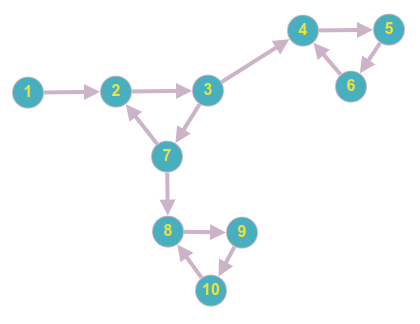
\includegraphics[scale=0.8]{prog_test/multiple_cycles_graph.png}}
	\caption{Некоторый граф, содержащий циклы.}
\end{figure}

Результатом работы программы на этих входных данных будет являться следующая последовательность вершин и соответствующий ей набор рёбер, разрезающих циклы.

\begin{figure}[h!]
	\center{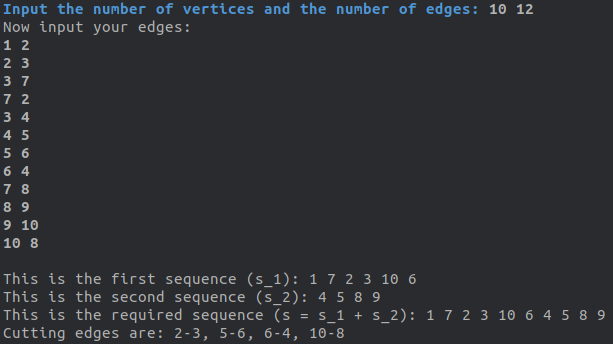
\includegraphics[scale=0.8]{prog_test/multiple_cycles_graph_output.png}}
	\caption{Полученная последовательность вершин и набор рёбер.}
\end{figure}

Видно, что в набор рёбер, разрезающих циклы, попало два ребра из одного цикла.  Возникающие в процессе вычисления неточности являются следствием 
использования приближённого алгоритма.

\par Полученные в результате применения приближённого алгоритма ациклические подграфы исходного графа могут отличаться от максимального ациклического
подграфа не более, чем в два раза.

\section*{Оценка сложности алгоритма}
\addcontentsline{toc}{section}{Оценка сложности}

\par Оценим временную сложность полученного приближённого алгоритма. Будем оценивать временную сложность каждого шага, проделываемого алгоритмом:

\par \textbf{Шаг 1.1. Поиск и выбор стока в графе.} Рассматриваемый блок кода:

\begin{lstlisting}[caption={Блок кода, отвечающий за поиск стока.},style=listingStyle, mathescape=true, language=C++]
while ((vertexPlaceholder = extractSink (graph)) != -1)
\end{lstlisting}

\textit{Стоком} в графе называется вершина, не имеющая выходящих из неё рёбер. В случае представления графа матрицей это означает, что строка этой 
вершины в матрице смежности содержит только нули (поскольку граф невзвешенный, то единица в матрице смежности означает наличие между вершинами ребра, 
а ноль -- его отсутствие). В худшем случае для поиска стока необходимо осуществить  полный проход по матрице, что указывает на временную сложность
$O(n^2)$, где $n$ -- число вершин в графе.

\par \textbf{Шаг 1.2. Редукция матрицы.} Рассматриваемый блок кода:

\begin{lstlisting}[caption={Блок кода, отвечающий за редукцию матрицы.},style=listingStyle, mathescape=true, language=C++]
reduceMatrix (vertexPlaceholder);, $\text{расположенный внутри}$
while ((vertexPlaceholder = extractSink (graph)) != -1)
\end{lstlisting}

После нахождения стока необходимо обновить матрицу смежности графа так, чтобы найденная вершина не использовалась
в дальнейших вычислениях. Это достигается путём помещения значения -1 в строку и столбец найденного стока. Общее число операций для первого найденного
стока составляет $2n - 1$ и, следовательно, оценка сложности -- $O(n)$. 

\par \textbf{Шаг 1.3. Промежуточная проверка графа на пустоту.} Рассматриваемый блок кода: 

\begin{lstlisting}[caption={Блок кода, отвечающий за поиск стока.},style=listingStyle, mathescape=true, language=C++]
if (adjacencySum () == negGrSizeSq)
	break;
\end{lstlisting}

В данной реализации граф считается пустым, если каждая ячейка 
его матрицы смежности содержит -1. Для вычисления необходимого значения нужно пройти каждую ячейку матрицы и добавить значение, хранящееся в ней, в 
аккумулятор. Временная сложность -- $O(n^2)$.

\par \textbf{Шаг 2.1. Поиск и выбор истока в графе.} Рассматриваемый блок кода:

\begin{lstlisting}[caption={Блок кода, отвечающий за поиск стока.},style=listingStyle, mathescape=true, language=C++]
while ((vertexPlaceholder = extractSource (graph)) != -1)
\end{lstlisting}
 
\textit{Истоком} в графе называется вершина, не имеющая входящих в неё рёбер. В случае представления графа матрицей это означает, что столбец этой 
вершины в матрице смежности содержит только нули. Дальнейшие рассуждения аналогичны полученным на шаге 1.1. Временная сложность -- $O(n^2)$.

\par \textbf{Шаг 2.2. Редукция матрицы.} Аналогично шагу 1.2.

\par \textbf{Шаг 2.3. Промежуточная проверка графа на пустоту.} Аналогично шагу 1.3.

\par \textbf{Шаг 3.1. Получение вершины с оптимальным $\delta$.} Рассматриваемый блок кода: 

\begin{lstlisting}[caption={Блок кода, отвечающий за поиск стока.},style=listingStyle, mathescape=true, language=C++]
vertexPlaceholder = getMaxDeltaVertex ();
\end{lstlisting}

Осуществляется проходом по непустой части графа. Для каждой вершины просматривается соответствующие этой вершине столбец и строка. В худшем случае 
для каждой из $n$ вершин необходимо просмотреть $2n - 1$ значений ячеек её столбца и строки. Временная сложность -- $O(2n^2 - n) = O(n^2)$.

\par \textbf{Шаг 3.2. Редукция матрицы.} Аналогично шагам 1.2 и 2.2.

Получаем, что общая временная сложность внутренней части цикла равна $O(n^3 + n^3 + n^2 + n^2) = O(n^3)$. Однако сама проверка выполнения условия цикла
требует выполнения $n^2$ операций, из чего следует, что временная сложность приближённого алгоритма составляет $O(n^5)$ -- полиномиальная временная 
сложность.

\conclusion

В ходе данной лабораторной работы был рассмотрен вопрос о сведении задачи о вершинном покрытии к задаче о нахождении множества рёбер, разрезающих циклы.
Был рассмотрен псевдокод приближённого алгоритма и осуществлена его программная реализация. Также была дана оценка временной сложности приближённого 
алгоритма.

\newpage

\begin{thebibliography}{1}
\bibitem{heurist} Eades, P., Lin, X. and Smyth, W.F. (1993) A fast and effective heuristic for the feedback arc set problem. Information Processing Letters, 47 (6). pp. 319-323.
\end{thebibliography}

\end{document}
